% Specify the type of document
\documentclass[12pt]{article}

% Load a number of useful packages
\usepackage{graphicx}
\usepackage{amsmath,amssymb,amsfonts,amsthm}
\usepackage{commath}
\usepackage{gensymb}
\usepackage[margin=1.0in]{geometry}
\usepackage[colorlinks=true]{hyperref}
\usepackage{cite}
\usepackage{hyperref}
\hypersetup{colorlinks,linkcolor={blue},citecolor={teal},urlcolor={red}}  
\usepackage[caption=false,font=footnotesize]{subfig}
\usepackage{wrapfig}

% Two more packages that make it easy to show MATLAB code
\usepackage[T1]{fontenc}
\usepackage[framed,numbered]{matlab-prettifier}
\lstset{
	style = Matlab-editor,
	basicstyle=\mlttfamily\small,
}


% Say where pictures (if any) will be placed
\graphicspath{{./pictures/}}

% Define title, author, and date
\title{AE353: Design Problem 04}
\author{Two-Wheel Robotics}
\date{April 11, 2019}

% Start of document
\begin{document}

% Put the title, author, and date at top of first page
\maketitle

\section{Goal} \label{sec:1}
\begin{wrapfigure}[8]{r}{0.45\textwidth}
\vspace{-6em}%
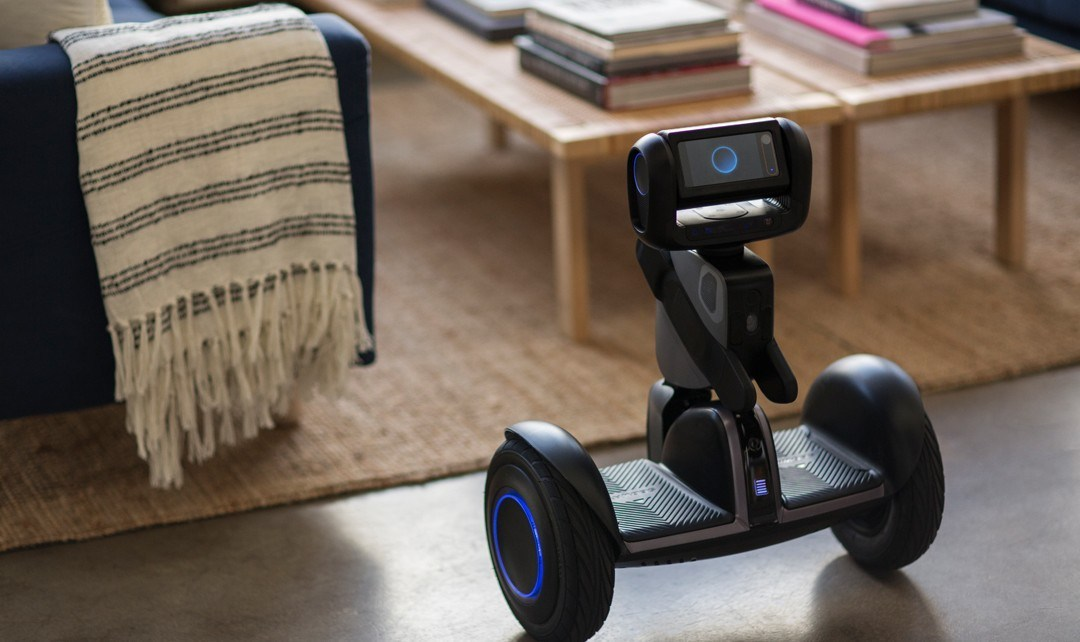
\includegraphics[width=0.4\textwidth]{segwayrobotics.jpg}
\vspace{-1em}
\caption{Modern robot friend by Segway (\href{https://macsources.com/segway-robotics-defines-the-future-of-mobile-robots-with-loomo-news/}{Photo from Mac Sources}). \label{figure:1}}
\end{wrapfigure}

This simulation will follow the life of a two-wheeled robot -- known as Bobby -- as it utilizes its individually torque-powered wheels to follow a generated path in Matlab.  The robot is equipped with two actuators which control $\tau_R$ and $\tau_L$, the torque of the individual wheels and a smart sensors which tracks lateral error, heading error, the radius of curvature of the road, and the angular velocity of each wheel.

\subsection{Requirements} \label{sec:1.1}
The robot is required to reach and maintain a forward-oriented velocity of $3 \frac{\mbox{m}}{\mbox{s}}$.  The robot must not crash, diverge from path, or exceed a pitch angle of $\phi = 30\degree$ in order to maintain optimal speed and stability.

\subsection{Verification} \label{sec:1.2}
The simulation will contain a verification test to ensure the requirements are satisfied.  This will be done by checking if $v \geq 3 \frac{\mbox{m}}{\mbox{s}}$.  The \lstinline{processdata.v} vs. \lstinline{processdata.t} will be plotted to verify whether the robot met the desired velocity within the time requirement.

\section{Model} \label{sec:2}
The system of non-linearized ODE's defining the equations of motion are provided as\\ \lstinline{DesignProblem04_EOMs.mat} and will be accessed in conjunction with \lstinline{fsolve()} and \lstinline{jacobian()} functions to determine equilibrium points and state space model.  Three separate controller tests will be created: slow, speed, optimized speed.  The slow test will verify the robot's controller can successfully allow navigation at slow speeds; the speed test will attempt to make the robot reach the required speed but will likely fail offering valuable information for future tests; the optimized speed test will satisfy the requirements.

\subsection{Robot Dynamics} \label{sec:2.1}
In general, the non-linearized differential system may be defined as shown in eqn \ref{eqn:1}:
\begin{equation} \label{eqn:1}
    \begin{aligned}
    \begin{bmatrix}
        \ddot{\phi} \\ \dot{v} \\ \dot{w}
    \end{bmatrix} &= f(\phi, \dot{\phi}, v, w, \tau_R, \tau_L), \quad
    \mbox{State} &&= 
    \begin{bmatrix}
        \dot{\phi} - \dot{\phi}_E \\ v - v_E \\ w-w_E \\ \phi - \phi_E \\ e_{lateral} - e_{lateral,E} \\ e_{heading} - e_{heading, E}
    \end{bmatrix} \\
    \mbox{Input} &=
    \begin{bmatrix}
        \tau_R - \tau_{R,E} \\ \tau_L - \tau_{L,E}
    \end{bmatrix}, \qquad \enspace \enspace
    \mbox{Output} &&= 
    \begin{bmatrix}
        e_{lateral} - e_{lateral,E} \\ e_{heading} - e_{heading, E}
    \end{bmatrix}
    \end{aligned}
\end{equation}
Each of the variables correspond to the following real-life values as defined in table \ref{tbl:1}
\begin{equation} \label{tbl:1}
\begin{array}{|c c| c c|}
    \hline
    \phi \rightarrow & \mbox{Chassis Angle} & \dot{\phi} \rightarrow & \mbox{Change in Chassis Angle} \\ \hline
    v \rightarrow & \mbox{Forward Velocity} & w \rightarrow & \mbox{Turning rate}\\ \hline
    \tau_L \rightarrow & \mbox{Left Motor Torque} & \tau_R \rightarrow & \mbox{Right Motor Torque}\\ \hline
\end{array}
\end{equation}

The simulator is designed to accept three equations of motion in reference to the position of the robot, $(x, y) \mbox{ and } \theta$, defined by (\ref{eqn:3}):
\begin{equation} \label{eqn:3}
    \begin{aligned}
        \dot{x} &= v\cos{\theta} \\
        \dot{y} &= v\sin{\theta} \\
        \dot{\theta} &= w
    \end{aligned}
\end{equation}
In order to let the robot keep track of the centerline of the road, equation (\ref{eqn:4}) is implemented to provide a method of letting the robot mitigate the error between robot position and the centerline.  Additionally, \ref{eqn:5} outlines the effects of the two $\omega$ values \cite{TAM212}:

\begin{equation} \label{eqn:4}
    \begin{aligned}
        w_{road} &= \frac{v_{road}}{r_{road}} \\
        \dot{e}_{lateral} &= -v\sin(e_{heading}) \\
        \dot{e}_{heading} &= w - (\frac{v \cos(e_{heading})}{v_{road} + w_{road}e_{lateral}})w_{road}
    \end{aligned}
\end{equation}
\begin{equation} \label{eqn:5}
    \omega_R = \frac{(v + \frac{\omega b}{2})}{r}, \quad \omega_L = \frac{(v - \frac{\omega b}{2})}{r}
\end{equation}

\subsection{Equilibrium Values} \label{sec:2.2}
In order to find equilibrium values which best fit the \hyperref[sec:1.1]{requirements}, the following values in table \ref{tbl:2} were selected for the first and second trials:
\begin{equation} \label{tbl:2}
    \begin{array}{|c|c|c|c|c|c|c|c|c|c|}
    \hline
    \dot{\phi} & v & w & \phi & e_{lateral} & e_{heading} & \tau_R & \tau_L & r_{road} & v_{road} \\ \hline
    0 & 2 & 0 & 0 & 0 & 0 & 0 & 0 & \infty & 2 \\ \hline
    0 & 3 & 0 & 0 & 0 & 0 & 0 & 0 & \infty & 2 \\ \hline
    \end{array}
\end{equation}

\subsection{State Space Model} \label{sec:2.3}
By use of the \lstinline{fsolve()} to find equilibrium values and \lstinline{jacobian()} to find the coefficients for the state-space matrix, the generalized State Space model may be defined as shown in \ref{eqn:6}:
\begin{equation} \label{eqn:6}
\begin{aligned}
    \dot{m} &= Am + Bu \\ n &= Cm + Du
\end{aligned}
\end{equation}
While there were three different controllers, the difference among trials arose from modifying the gain matrix for LQR.  The coefficients, A, B, and C may be found in \ref{eqn:7}:

\begin{equation} \label{eqn:7}
    A = \begin{bmatrix}
    0 & 0 & 0 & 27.0 & 0 & 0\\ 0 & 0 & 0 & -3.5 & 0 & 0\\ 0 & 0 & 0 & 0 & 0 & 0\\ 1.0 & 0 & 0 & 0 & 0 & 0\\ 0 & 0 & 0 & 0 & 0 & -3.0\\ 0 & 0 & 1.0 & 0 & 0 & 0
    \end{bmatrix}, \enspace
    B = \begin{bmatrix} -2.2 & -2.2\\ 0.59 & 0.59\\ 2.5 & -2.5\\ 0 & 0\\ 0 & 0\\ 0 & 0 \end{bmatrix}, \enspace
    C = \begin{bmatrix} 0 & 0 & 0 & 0 & 1.0 & 0\\ 0 & 0 & 0 & 0 & 0 & 1.0\\ 0 & 5.0 & 1.0 & 0 & 0 & 0\\ 0 & 5.0 & -1.0 & 0 & 0 & 0 \end{bmatrix}
\end{equation}

\section{Controller Design} \label{sec:3}
\subsection{Controller} \label{sec:3.1}
To begin implementing the controller, the input must first be defined as in \ref{eqn:8}:
\begin{equation} \label{eqn:8}
    u = -Km
\end{equation}
In order to find an optimized K value, the data found in \hyperref[sec:2.3]{Section 2.3}
will be used with a gain matrix to evaluate \lstinline{K = lqr}$(A, B, Q_c, R_c)$.
It is very important to note the Controller gains ratio is extremely sensitive and can result in critical failure depending on initial values.  The open loop controllability may be tested by determining the full-rank and condition of the controllability matrix, \lstinline{cond(ctrb(A,B)); rank(ctrb(A,B))}.  Closed-loop asymptotic stability was verified by use of finding all \lstinline{eig(A-BK)} values negative.  The controller was successfully verified as controllable and asymptotically stable.
\subsection{Observer} \label{sec:3.2}
Since the only sensors equipped on the robot are $e_{lateral}, e_{heading}, \omega_R, \omega_L, \mbox{ and } r_{road}$, it is crucial to create an observer.  This may be done by first finding an optimized value for L by \lstinline{L = lqr}$(A', C', R^{-1}_o, Q^{-1}_o)$.  The ultimate observer is designed as follows in \ref{eqn:9}:
\begin{equation} \label{eqn:9}
    \hat{\dot{m}} = A\hat{m} + Bu - L(C\hat{m} - n)
\end{equation}
In order to determine the open-loop observability, the condition number and rank may be used by finding \lstinline{cond(obsv(A, C)); rank(obsv(A,C))}.  The closed-loop asymptotic stability may be verified by determining the signs of \lstinline{eig(A-LC)}.  Both were verified and therefore the observer is both observable and asymptotically stable.

\section{Simulation Tests} \label{sec:4}
With the observer and controller completed, the two actuators may be assigned as follows: \lstinline{actuators.tauR = u(1) + tauRE; actuators.tauL = u(2) + tauLE} for $\tau_{RE} \mbox{ and } \tau_{LE}$ equilibrium values for $\tau$.  Since both conditions numbers were on the order of magnitude of $e4$ and $e3$, a relatively high ratio of $\frac{Q}{R}$ will need to be implemented.

\subsection{Trial 1} \label{sec:4.1}
In the first, slower trial, a low equilibrium velocity of $v = 2$ meters per second was designated to analyze whether the controller and observer operate nominally.  The results were positive with an operational robot tracking the road.

\subsection{Trial 2} \label{sec:4.2}
\begin{wrapfigure}[8]{r}{0.3\textwidth}
\vspace{-6em}%
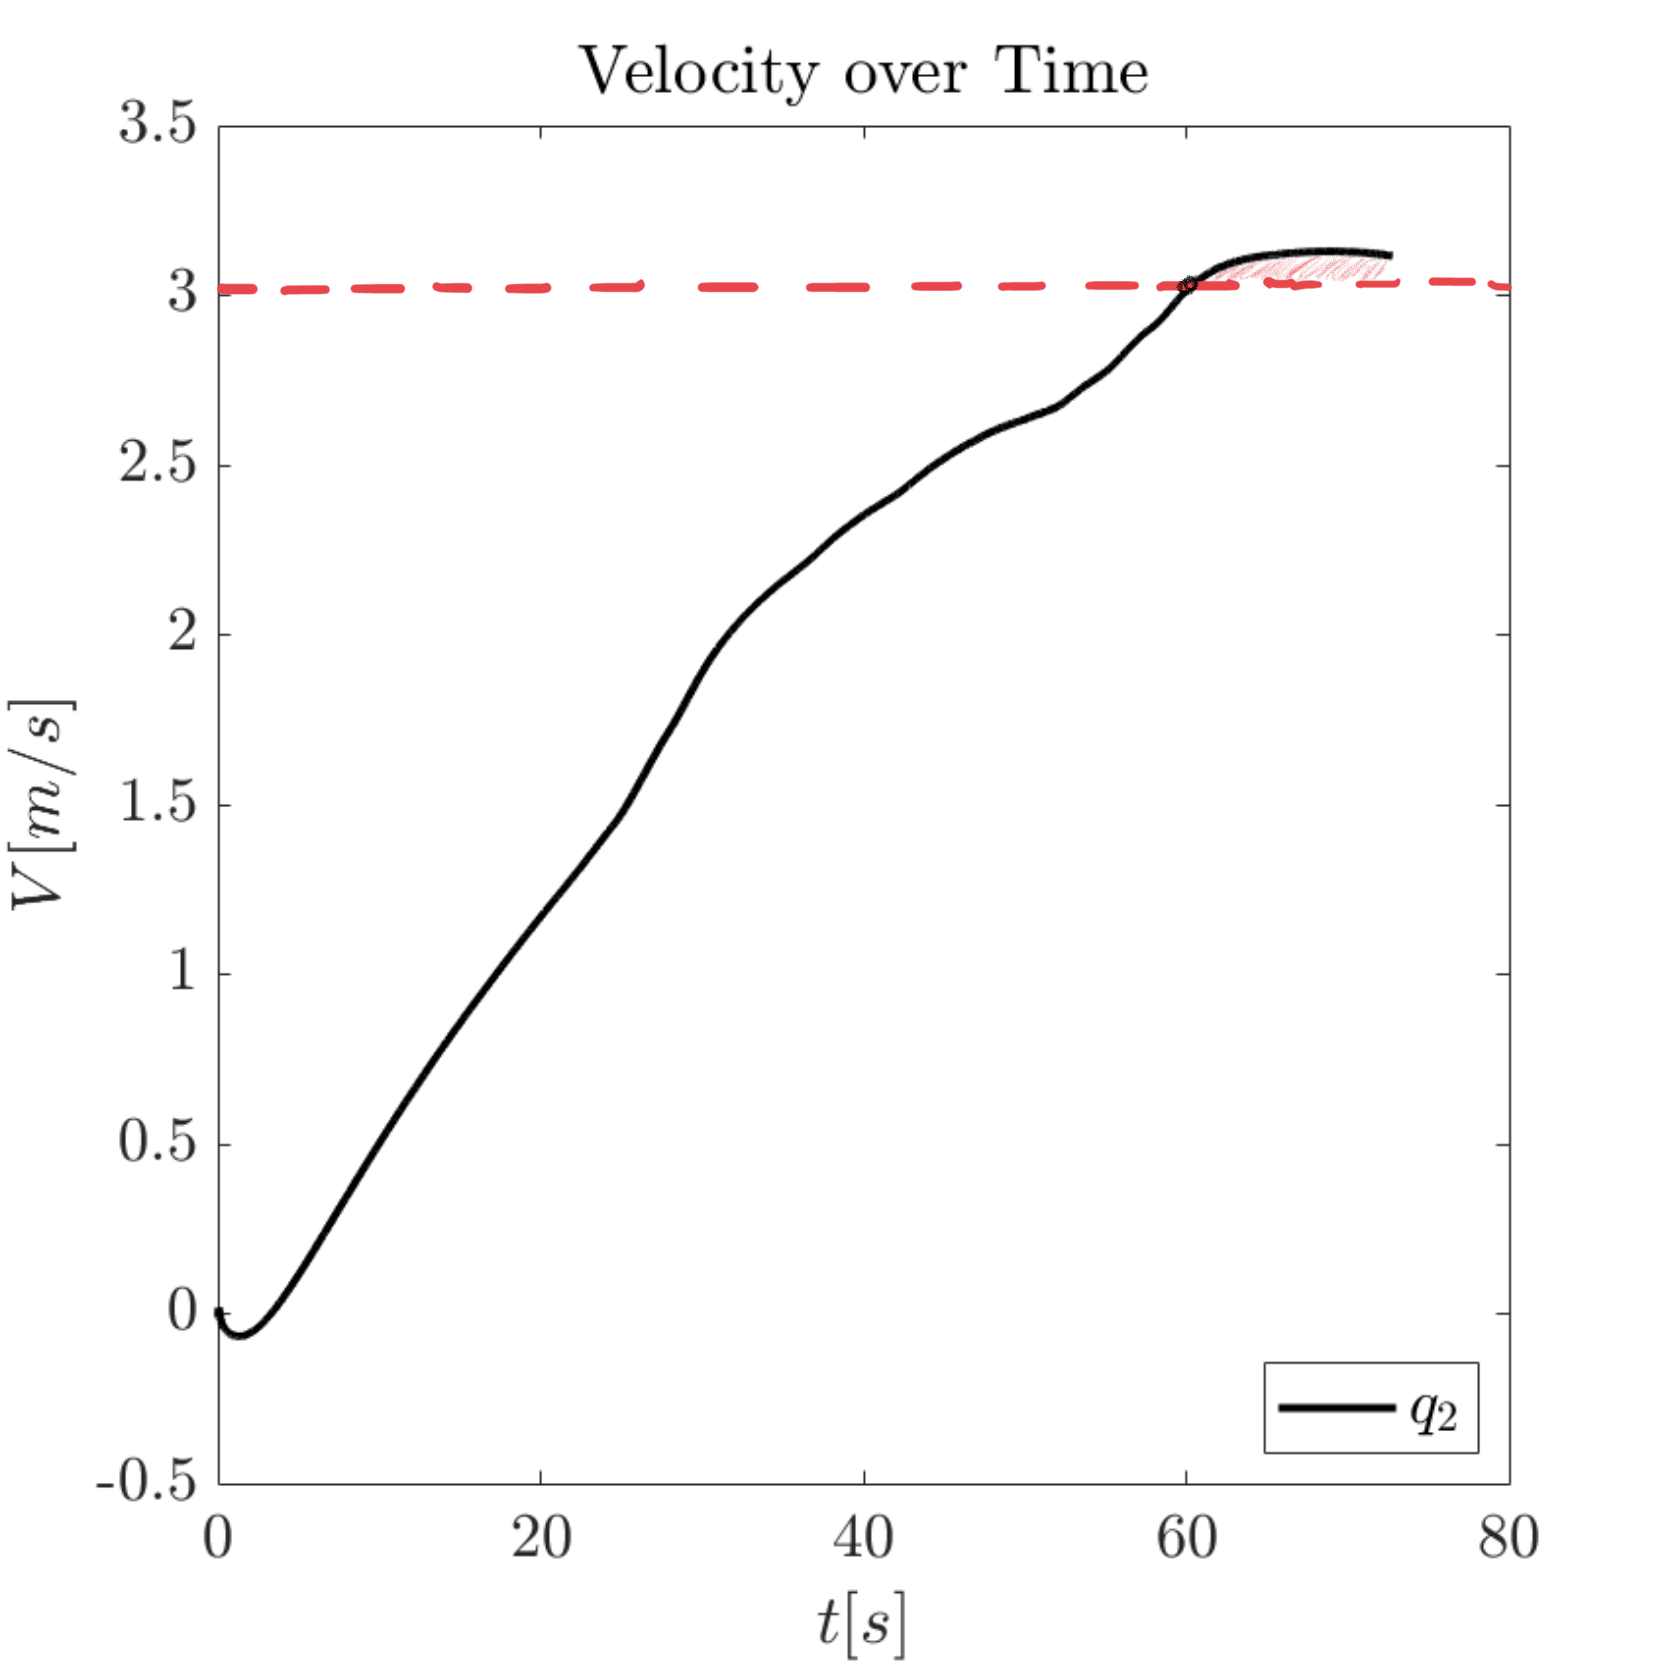
\includegraphics[width=0.3\textwidth]{File_001.png}
\vspace{-2em}
\caption{\tiny{Trial 3 Successful Velocity} \label{figure:2}}
\end{wrapfigure}
As the equilibrium value was bumped up to the required velocity of $v = 3$ meters per second, the robot successfully tracked the majority of the road but failed whenever the robot reached a double-bend or $180\degree$ turn, indicating the controllability matrix was not powerful enough to provide quicker reactions to the actuators.  Hypothesis: increasing K value by changing the $\frac{Q_c}{R_c}$ ratio will let the robot properly adjust the actuators.

\subsection{Trial 3} \label{sec:4.3}
Inspiration for a modified $I$ matrix was shown in \cite{Bonafilia} and provided a useful matrix designation for $Q_c$, resulting in a stable and efficient K value.  The Q matrix is defined by \ref{eqn:10}:
\begin{equation} \label{eqn:10}
    Q_c = 
    \begin{bmatrix}
        6\cdot 10^4 & 0 & 0 & 0 & 0 & 0 \\
        0 & 1 & 0 & 0 & 0 & 0 \\
        0 & 0 & 1 & 0 & 0 & 0 \\
        0 & 0 & 0 & 1 & 0 & 0 \\
        0 & 0 & 0 & 0 & 4\cdot 10^2 & 0 \\
        0 & 0 & 0 & 0 & 0 & 1
    \end{bmatrix}, \qquad R_c = 200\cdot \begin{bmatrix} 1 & 0 \\ 0 & 1 \end{bmatrix}
\end{equation}
This resulted in a significantly more stable controller, capable of reaching the required speed and passing the verification.  




% Display list of references in IEEE format.
\bibliographystyle{IEEEtran}
\bibliography{IEEEabrv,references}
\end{document}